\documentclass{SGGW-thesis}

\INZYNIERSKAtrue
\WZIMtrue

\title{Zastosowanie metod uczenia maszynowego do stworzenia sztucznej inteligencji w turowych grach RPG}
\Etitle{The use of machine learning methods to create artificial intelligence in turn-based RPG games}
\author{Rafał Kuligowski}
\date{2023}
\album{205835}
\thesis{Praca dyplomowa na kierunku:}
\course{Informatyka}
\promotor{dra Marka Karwańskiego}
\pworkplace{Instytut Informatyki Technicznej\\Katedra Zastosowań Matematyki}

\renewcommand{\thefigure}{\arabic{figure}}
\usepackage[bottom]{footmisc}
\usepackage{hyperref}
\usepackage{subfigure}
\usepackage{float}
\usepackage{listings}
\usepackage{cite}
\raggedbottom

\begin{document}
\maketitle
\statementpage
\abstractpage
{Zastosowanie metod uczenia maszynowego do stworzenia sztucznej inteligencji w turowych grach RPG}
{Tematem pracy było zaimplementowanie sztucznej inteligencji uczącej się za pomocą metod uczenia maszynowego w turowej grze RPG. Praca składa się z czterech głównych części.
Pierwsza część omawia technologie wykorzystane w pracy oraz ich alternatywy. Druga część skupia się na implementacji wcześniej wspomnianych technologii.
Trzecia część zawiera instrukcję użytkowania gotowej aplikacji. W czwartej części znajdują się wnioski dotyczące implementacji tematycznego rozwiązania w produktach komercyjnych.}
{uczenie maszynowe, sztuczna inteligencja, gry RPG, uczenie przez wzmacnianie, turowe systemy walki}
{The use of machine learning methods to create artificial intelligence in turn-based RPG games}
{The topic of the paper was the implementation of artificial intelligence, which learns through machine learning methods, in a turn-based RPG game. 
The paper consists of four main parts. The first part discusses the technologies used in the work and their alternatives. The second part focuses on 
the implementation of the aforementioned technologies. The third part contains user instructions for the finished application. The fourth part includes 
conclusions regarding the implementation of the thematic solution in commercial products.}
{machine learning, artificial intelligence, RPG games, reinforcement learning, turn-based battle system}


{
  % Spis treści może być złożony z pojedynczą interlinią, np. jeśli jedna linia wychodzi na następną stronę.
  % W przeciwnym razie spis treści wstawić bez powyższego rozkazu i klamry.
  \doublespacing
  \tableofcontents
}

\startchapterfromoddpage % niezależnie od długości spisu treści pierwszy rozdział zacznie się na nieparzystej stronie

\chapter{Wstęp}
Sztuczna inteligencja w ciągu ostatnich lat objęła wiele dziedzin życia i ciągle dynamicznie się rozwija. 
Jej zastosowanie jest bardzo rozległe, a jedną z branż o dużych perspektywach rozwoju tej technologii jest przemysł rozrywkowy, 
w który wchodzą gry wideo. W grach można zastosować tę technologię do generowania misji i zadań dla graczy, aby nie były one powtarzalne, 
stworzenia mądrego systemu automatycznej walki, dzięki któremu gracz nie lubiący tego elementu w grze może go pominąć, oraz do stworzenia 
sztucznej inteligencji dla przeciwników gracza. Ostatnie z tych przykładowych zastosowań zostanie omówione pod względem teoretycznym i praktycznym 
zgodnie z tematem pracy.

\section{Cel i zakres pracy}
Praca ma na celu zbadanie możliwości implementacji sztucznej inteligencji dla przeciwników w grach wideo z gatunku RPG\footnote{RPG (ang. Role Playing Games)
- gry, w których gracz wciela się w rolę postaci występujących w fikcyjnym świecie. Gracze ponoszą wszelkie konsekwencje swoich akcji jako postać w świecie gry.}
z turowym systemem walki. Wynikiem pracy będą dwie aplikacje: jedna trenująca model, a druga testująca model w postaci symulatora walki. 
Treść pracy będzie stanowić opisy technologii użytych w pracy wraz z alternatywami, opis implementacji rozwiązania na podstawie wybranych 
wcześniej technologii, instrukcję obsługi napisanej aplikacji oraz wnioski na temat implementacji takiego rozwiązania w grach komercyjnych na 
podstawie tego projektu.

\chapter{Technologie}
W tym rozdziale zostaną szczegółowo omówione komponenty potrzebne do implementacji takiej sztucznej inteligencji. Według kolejności wyboru są to: 
\begin{itemize}
  \item{Rodzaj uczenia maszynowego}
  \item{Silnik do stworzenia gry oraz pakiet do uczenia maszynowego kompatybilny z silnikiem}
  \item{Wykorzystywany algorytm do uczenia maszynowego}
  \item{System walki (w przypadku tej pracy - system oparty o tury)}
\end{itemize}


\section{Rodzaje uczenia maszynowego}
W uczeniu maszynowym można rozróżnić trzy jego główne rodzaje (w oparciu o drugi rozdział z~\cite{MachineLearningTypes}):
\begin{itemize}
  \item{Nadzorowane (ang. Supervised) - model jest trenowany na danych wejściowych oraz odpowiednich dla nich wartości wynikowych. Na ich podstawie uczy się przewidywania wyniku dla nowych, nieznanych danych wejściowych.}
  \item{Nienadzorowane (ang. Unsupervised) - model jest trenowany na samych danych wejściowych nie dostając oczekiwanych wyników. Model sam musi odkryć sens jaki stoi za danymi wejściowymi.}
  \item{Przez wzmacnianie (ang. Reinforcement) - model trenowany za pomocą interakcji trenowanego agenta z wykreowanym otoczeniem. Agent wykonując akcje w otoczeniu dostaje nagrody lub kary w zależności od wyników jego akcji.}
\end{itemize}
W przypadku tej pracy zostanie użyty rodzaj uczenia przez wzmacnianie, z uwagi na charakterystyczną dla niego metodę uczenia przez interakcje. 
Metoda ta pasuje do gier wideo, gdyż z założenia polegają one na interakcji gracza ze światem gry. Model będzie mógł, tak jak gracz grający w grę, 
poprzez ingerencję za pomocą akcji w otoczenie, uczyć się wykonywania najlepszych możliwych akcji w danym momencie. Więcej informacji na temat 
działania uczenia przez wzmacnianie zawarto w~\cite{ReinforcementLearning}.

\section{Silniki graficzne oraz pakiety do uczenia}
Wybór silnika graficznego oraz pakietu do uczenia maszynowego jest głęboko powiązany. Ponadto jest to kwestia mocno subiektywna, gdyż zależy od umiejętności autora projektu. Oto lista niektórych wyborów w zakresie silnika i pakietu do uczenia maszynowego:
\subsection{Unity z pakietem ML-Agents}
Wśród wymienionych gotowych pakietów, ML-Agents jest najstarszym rozwiązaniem (udostępnione w 2017r.\footnote{Repozytorium powstało 8.09.2017r, pierwsza wersja pakietu pochodzi z 16.09.2017r - link do repozytorium \url{https://github.com/Unity-Technologies/ml-agents}}).
Dostępne w pakiecie są 2 algorytmy uczenia przez wzmacnianie - PPO oraz SAC\footnote{Więcej informacji o tych algorytmach w rozdziale "\nameref{algorithms}"}. Pakiet posiada własną dokumentację\cite{MLAgentsDocs}. 
Sam silnik Unity umożliwia tworzenie aplikacji z grafiką 2D oraz 3D, operuje na łatwym w nauce języku C\# oraz ma rozbudowaną dokumentację\cite{UnityDocs}.
\subsection{Godot z pakietem RL Agents}
Godot jest silnikiem OpenSource o coraz mocniejszej pozycji na rynku. Według dokumentacji \cite{GodotDocs},
silnik wspiera oficjalnie 2 języki programowania: autorski język GDScript oraz C\#. Twórcy za pośrednictwem technologii GDExtension zapewnili możliwość dodania wsparcia dla innych języków przez społeczność.
Dzięki temu, można na tym silniku programować również w innych językach programowania takimi jak Rust, C++ czy Swift. Pakiet RL Agents jest najbardziej rozbudowanym pakietem wśród wymienionych.
Bazuje na 4 innych pakietach\footnote{Pakiety na których bazuje RL Agents - StableBaseLines3, SampleFactory, CleanRL oraz Ray rllib (stan na 06.01.2024r.)} do uczenia przez wzmacnianie
oraz wspiera ponad 12 algorytmów uczenia. Więcej informacji o RL Agents można znaleźć w artykule naukowym poświęconym tej technologii~\cite{GodotRLAgentsArticle} oraz w dokumentacji dostępnej w repozytorium projektu~\cite{GodotRLAgentsDocs}.
\subsection{Unreal Engine z pakietem Learning Agents}
W porównaniu do innych pakietów, Learning Agents jest najmłodszy (powstał na początku 2023r.) oraz najsłabiej udokumentowany. Pakiet operuje algorytmami PPO oraz BC (ang. Behavioral Cloning)\footnote{Informacja pochodzi ze źródła (stan na 06.01.2024r.): \url{https://dev.epicgames.com/community/learning/tutorials/8OWY/unreal-engine-learning-agents-introduction}}. 
Mimo to sam silnik Unreal Engine jest potężnym narzędziem z bardzo dużym wsparciem i możliwościami. Posiada wsparcie dla języka C++ oraz funkcji Blueprints umożliwiającej programowanie wizualne (bez pisania kodu). 
Dokumentacja zarówno silnika Unreal Engine jak i pakietu Learning Agents znajduje się w~\cite{UnrealDocs}.
\subsection{Własny silnik z wykorzystaniem różnych pakietów do uczenia maszynowego}
Rozwiązanie oferujące największą swobodę, ale też najtrudniejsze w implementacji. Do stworzenia środowiska gry potrzebna jest biblioteka graficzna pomagająca stworzyć silnik np. OpenGL
lub pakiet do stworzenia aplikacji okienkowej np. PyGame. Wybierając pakiet do uczenia maszynowego warto szukać wśród pakietów Pythona gdyż ma on ich bardzo dużo. Dla uczenia przez wzmocnienie można zastosować pakiet PyTorch\footnote{Używany w ML-Agents oraz Learning Agents}
lub też jeden z 4 pakietów wykorzystywanych przez RL Agents.
\subsection*{Wybrany silnik i pakiet do uczenia maszynowego}
Do pracy wybrałem Unity z pakietem ML-Agents przez moje wcześniejsze doświadczenie z Unity oraz zaawansowanie w języku C\#. Uważam jednak, że dużo bardziej rozbudowany RL Agents na silniku Godot jest lepszym wyborem do tego typu projektu, gdyż daje dużo większe pole do dostosowania uczenia dla osiągnięcia lepszych rezultatów.


\section{Algorytmy do uczenia maszynowego}
\label{algorithms}
Unity ML-Agents posiada 2 algorytmy uczące PPO (ang. Proximal Policy Optimization) oraz SAC (ang. Soft Actor-Critic). Pierwszy z nich jest podstawowym algorytmem używanym w pakiecie. Według \cite{MLAgentsDocs} algorytm PPO jest algorytmem ogólnego przeznaczenia i jest bardziej stabilny w porównaniu z innymi algorytmami uczenia przez wzmacnianie.
To samo źródło opisuje również różnicę między algorytmem SAC i PPO. SAC jest algorytmem "off-policy" kiedy PPO jest algorytmem "on-policy". Oznacza to że SAC uczy się z doświadczeń zebranych w dowolnym momencie w przeszłości, a podczas uczenia są losowo dobierane do treningu, gdzie w PPO występuje "policy",
które reguluje podejmowanie decyzji i jest ulepszane z każdą iteracją uczenia. Dodatkowe informacje o algorytmie PPO znajdują się w~\cite{PPOArticle}, a o SAC w~\cite{SACArticle}. 

\pagebreak
Do projektu wybrany został algorytm PPO z uwagi na wcześniej podaną stabilność oraz fakt, że jest on algorytmem będącym ponad 6 lat w pakiecie ML-Agents co sugeruje, że jest on lepiej rozwiniętym rozwiązaniem w pakiecie.

\section{Systemy walki w turowych grach RPG}
Systemów walki turowej w grach RPG jest bardzo dużo i każda gra, nawet opierając się o jakiś system, przerabia go tak aby stał się wyjątkowy. Pewne elementy jednak się nie zmieniają i można je zauważyć w każdej grze z tego gatunku:
\begin{itemize}
  \item{Rozgrywka polega na wymianie tur postaci gracza z przeciwnikami}
  \item{Podczas tury gracz oraz przeciwnicy wykorzystują swoje tury jako zasób do wykonywania akcji}
  \item{Postacie gracza oraz przeciwnicy posiadają statystyki, które określają ich cechy. Do takich statystyk może należeć np. Obrona zmniejszająca obrażenia otrzymywane przez postać, czy też Atak zwiększający zadawane obrażenia}
  \item{Postacie gracza oraz przeciwnicy posiadają umiejętności, których mogą używać zużywając tury do wykonywania akcji w środowisku gry}
  \item{Walka kończy się gdy wszystkie postacie gracza lub wszyscy przeciwnicy umrą}
\end{itemize}
Powyższe punkty zostały oparte o własne doświadczenia z grami tego gatunku, jak i o wybrane rozdziały z~\cite{RLLearningInTBRPG, PlayerPreferencesInRPGs}. Poniżej przedstawię parę róźnych podejść do walki w systemie turowym:
\subsection{RPG Maker}
RPG Maker to program Low-Code/No-Code do tworzenia gier RPG. System walki w nim użyty jest dobrą bazą do tworzenia innych, 
bardziej skomplikowanych systemów przez swoją prostotę. Na początku walki jest tworzona kolejka złożona z postaci występujących na scenie 
(zarówno wrogich jak i sojuszniczych), która jest posortowana według statystyki Szybkości. Im większa owa statystyka, tym postać jest wyżej w 
kolejce i szybciej wykona ruch. Po stworzeniu kolejki, gracz wybiera ruchy wszystkich sojuszniczych postaci, a po wyborze ruchu ostatniej postaci
system przechodzi przez kolejkę postaci uruchamiając wybrane przez gracza oraz sztuczną inteligencję przeciwników akcje. Po wszystkim, 
system daje graczowi ponowną możliwość wyboru umiejętności. System ten był również zaimplementowany w grach z serii Etrian Oddysey oraz 
pierwszych częściach Final Fantasy.
\subsection{Darkest Dungeon}
System walki w tej grze jest zmodyfikowaną wersją poprzedniego systemu, jednak wprowadza większą dynamikę. 
Gdy kolejka postaci zostanie stworzona oraz postać w drużynie gracza ma aktualnie swoją turę, gracz wybiera akcję, 
którą postać ma wykonać. Po jej wybraniu, postać wykonuje akcję i przechodzi na koniec kolejki, przekazując turę następnej postaci w 
niej się znajdującej. System ten został również użyty w grach Yakuza: Like a Dragon, Like a Dragon: Infinite Wealth czy Super Mario RPG.
\subsection{Active Time Battle}
System walki charakteryzuje się tym, że każda postać na początku zaczyna z pustym paskiem tury, ładowanym się w równych interwałach. 
Gdy tura jakiejś postaci zostanie w pełni naładowana, walka zatrzymuje się, a postacie z naładowaną turą wybierają akcję, jaką mają wykonać. 
Następnie pasek tury jest dalej ładowany. Gdy ładowanie dobiegnie do końca, postać wykona wybraną wcześniej akcję i resetuje ładowanie tury 
do wartości początkowej. System ten jest znany z gier Chrono Trigger, Child of Light oraz serii Final Fantasy.
\subsection{Press-Turn System}
Został stworzony i głównie jest używany w grach firmy Atlus począwszy od gry~\cite{SMT3}. System opiera się na zwiększeniu znaczenia tury jako zasobu poprzez rozdzielenie tur na zwykłe i "wciśnięte", oraz wprowadzenie oceny ruchu postaci.
Ocena opiera się na 2 powiązanych ze sobą kryteriach:
\begin{enumerate}
  \item{Rodzaj obrażeń - np. żywioły typu ogień, woda, ziemia itp.}
  \item{Relację postaci do użytego rodzaju obrażeń}
\end{enumerate}
Pierwotna implementacja systemu zawiera 6 typów relacji do rodzaju obrażeń:
\begin{enumerate}
  \item{Normalna}
  \item{Słabość}
  \item{Odporność}
  \item{Niewrażliwość}
  \item{Odbicie}
  \item{Absorpcja}
\end{enumerate}
\pagebreak
System na początku rozdziela fazę gracza oraz fazę przeciwnika. Na początku każdej fazy liczona jest liczba tur jaką posiada poruszają się strona, która zazwyczaj jest liczbą postaci po danej stronie wykluczając martwe postaci (istnieją wyjątki od tej reguły).
Poza liczeniem liczby tur jest tworzona kolejka postaci w której kolejności będą poruszały się postaci po danej stronie. Gdy postać aktualnie posiadająca ruch wykona akcję zaczyna się jego ocena, która zmienia ilość posiadanych przez stronę tur.
W zależności od oceny tury mogą być odejmowane lub "wciskane". Zasady oceny wyglądają następująco:
\begin{itemize}
  \item{Jeśli postać trafi w słaby punkt innej postaci lub trafi cios krytyczny oraz posiada 1 lub więcej zwykłych tur, zwykła tura jest "wciskana"}
  \item{Jeśli postać trafi w słaby punkt innej postaci lub trafi cios krytyczny oraz posiada same tury "wciśnięte", odejmowana jest "wciśnięta" tura}
  \item{Trafienie niebędące trafieniem krytycznym lub trafienie w inny niż Słabość typ relacji powodeje odjęcie tur o konkretną ich liczbę priorytetyzując tury wciśnięte}
  \item{Jeśli postać postanowi przeczekać turę, system zachowuje się tak samo jak przy trafieniu krytycznym lub trafieniu w słaby punkt}
\end{itemize}
Gdy stronie wykonującej akcje skończą się tury, następuje zmiana stron.

\subsection*{Wybrany system walki}
Do implementacji został wybrany system Press-Turn z gry \cite{SMT3}. Mimo swojego skomplikowania (co może spowodować dłuższy czas uczenia modelu) posiada on bardzo dużo ciekawych interakcji związanych z turami, które sztuczna inteligencja będzie mogła wykorzystać na swoją korzyść.


\chapter{Implementacja}
Aplikacja jest podzielona na 2 części: automatycznie trenującą model oraz testującą model w symulatorze walki.


\section{Część aplikacji testująca model}
Ta część aplikacji została zaimplementowana jako pierwsza w celu przygotowania systemu Press-Turn. Składa się z 3 scen Unity: MainMenu, CharacterCreator oraz BattleScene.

\subsection{Scena MainMenu}
Menu Główne składa się z 2 widoków: Panelu głównego oraz opcji. W panelu głównym są dostępne przyciski START, CONFIG oraz EXIT. START służy do uruchomienia kreatora postaci, CONFIG otwiera widok opcji, a EXIT służy do zamknięcia aplikacji\footnote{Przycisk zamknięcia aplikacji nie działa podczas testowania aplikacji na silniku, tylko gdy aplikacja zostanie wyeksportowana.}.
Widok opcji posiada suwaki zmieniające głośność muzyki oraz dźwięków w aplikacji i przycisk zapisujący ustawienia.

\begin{figure}[H]
  \hfill
  \subfigure[Widok panelu głównego]{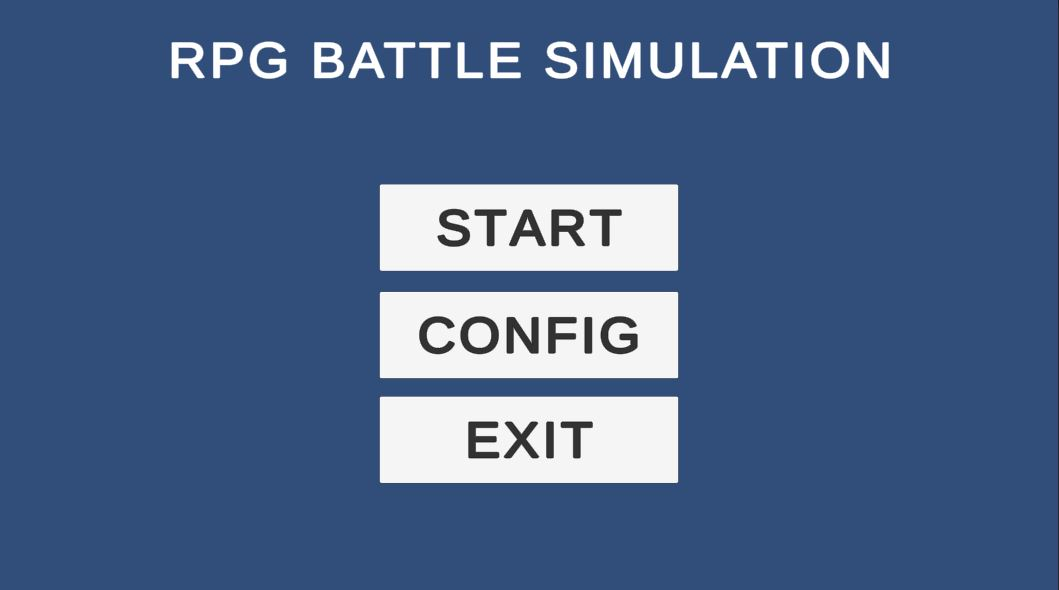
\includegraphics[width=1\textwidth]{menuscreen1.JPG}}
  \hfill
  \subfigure[Widok opcji]{
\includegraphics[width=1\textwidth]{menuscreen2.JPG}}
  \hfill
  \caption{Zrzuty ekranu przedstawiające menu główne}
\end{figure}
\pagebreak
\subsection{Scena CharacterCreator}
Kreator postaci składa się z 2 widoków: panelu wyboru liczby aktorów w drużynie oraz kreatora postaci. Oba widoki posiadają też przycisk BACK powracający do menu głównego.


\subsubsection{Panel wyboru liczby aktorów}
Panel składa się z suwaka przyjmującego wartości całkowite w zakresie 1-4 oraz przycisk potwierdzający ilość aktorów o treści ACCEPT. Po jego wciśnięciu widok zmienia się na kreator postaci.

\subsubsection{Kreator postaci}
Składa się z przycisku Restart Actors wracającego do widoku wyboru liczby aktorów, przycisku Start Battle zaczynającego walkę gdy wszyscy aktorzy mają wypełnione pola statystyk, pola wyboru aktualnie edytowanego aktora oraz obszernego ekranu do wprowadzania statystyk postaci.
Lista statystyk postaci (sens statystyk zostanie wyjaśniony podczas omawiania sceny walki):
\begin{enumerate}
  \item{HP (ang. Health Points, pl. Punkty Życia) - zakres 1-9999}
  \item{MP (ang. Mana Points, pl. Punkty Many) - zakres 1-9999}
  \item{Strength (pl. Siła) - zakres 1-99}
  \item{Magic (pl. Magia) - zakres 1-99}
  \item{Dexterity (pl. Sprawność) - zakres 1-99}
  \item{Agility (pl. Zwinność) - zakres 1-99}
  \item{Luck (pl. Szczęście) - zakres 1-99}
\end{enumerate}
\pagebreak
Postacie posiadają również Elementy i odpowiadające im relacje. Lista Elementów (kolejność od lewej według ustawienia w widoku):
\begin{enumerate}
  \item{Obrażenia fizyczne}
  \item{Ogień}
  \item{Lód}
  \item{Wiatr}
  \item{Elektryczność}
  \item{Światłość}
  \item{Ciemność}
  \item{Nadzwyczajny - ukryty element, zawsze o relacji neutralnej}
\end{enumerate}
Lista relacji Elementu z postacią (wraz ze skrótem widocznym w kreatorze, wpływem na tury oraz wpływem na obrażenia):
\begin{enumerate}
  \item{Neutralny, skrót: "-", wpływ na turę: utrata 1 tury, wpływ na obrażenia: brak}
  \item{Słabość, skrót: "Wk", wpływ na turę: "wciśnięcie" 1 tury, wpływ na obrażenia: +20\%}
  \item{Odporność, skrót: "Str", wpływ na turę: utrata 1 tury, wpływ na obrażenia: -20\%}
  \item{Niewrażliwość, skrót: "Null", wpływ na turę: utrata 2 tur, wpływ na obrażenia: zniwelowanie obrażeń}
  \item{Odbicie, skrót: "Rep", wpływ na turę: utrata 4 tur, wpływ na obrażenia: odbicie wartości obrażeń (obrażenia odbite również podlegają ocenie, ale nie wpływają na tury oraz nie mogą odbić się drugi raz)}
  \item{Absorbcja, skrót: "Abs", wpływ na turę: utrata 4 tur, wpływ na obrażenia: wyleczenie o wartość obrażeń}
\end{enumerate}
W skład kreatora wchodzi również lista z wyborem umiejętności. Każdy rekord listy posiada: pole wyboru umiejętności, jej nazwę, koszt oraz przypisany Element.
\pagebreak
\begin{figure}[H]
  \hfill
  \subfigure[Widok panelu wyboru liczby aktorów]{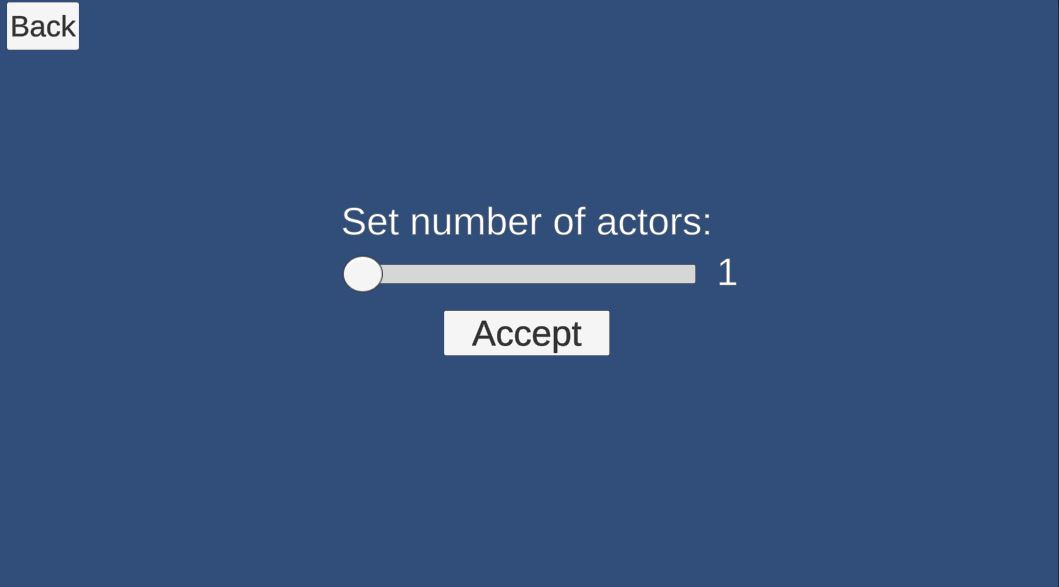
\includegraphics[width=1\textwidth]{creatorscreen1.JPG}}
  \hfill
  \subfigure[Widok kreatora postaci]{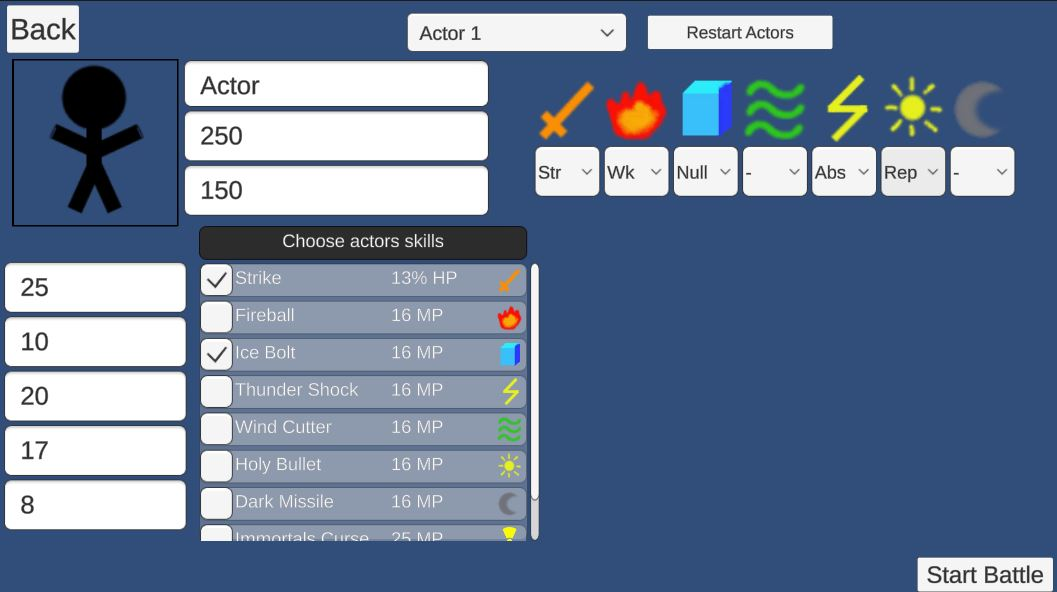
\includegraphics[width=1\textwidth]{creatorscreen2.JPG}}
  \hfill
  \caption{Zrzuty ekranu przedstawiające kreator postaci}
\end{figure}
\pagebreak
\subsection{Scena BattleScene}
Rozbudowana scena przedstawiająca informacje na temat aktualnego stanu walki. Stworzona na podstawie UI z gry~\cite{SMT3}.
Scena posiada następujące elementy UI:
\begin{itemize}
  \item{Przycisk Leave Battle - służy do wyjścia z walki}
  \item{Lista tur - czerwone znaczniki oznaczają "wciśnięte" tury, a zielone zwykłe tury}
  \item{Widok drużyny gracza - generowany automatycznie, obramowanie pokazuje kto aktualnie posiada ruch}
  \item{Widok przeciwnika - sterowany przez wytrenowany model przeciwnik z widocznym paskiem zdrowia}
  \item{Lista umiejętności - umożliwia wybór umiejętności aktualnie ruszającej się postaci. Po wyborze umiejętności gracz jest proszony o cel.}
  \item{Dziennik zdarzeń walki - pokazuje umiejętności użyte od początku walki przez jakąkolwiek postać}
  \item{Stan drużyny gracza - pokazuje paski z imionami wszystkich postaci gracza, jak i ich stanem zdrowia i many}
\end{itemize}
\begin{figure}[H]
  \hfill
  \subfigure[UI gry~\cite{SMT3}]{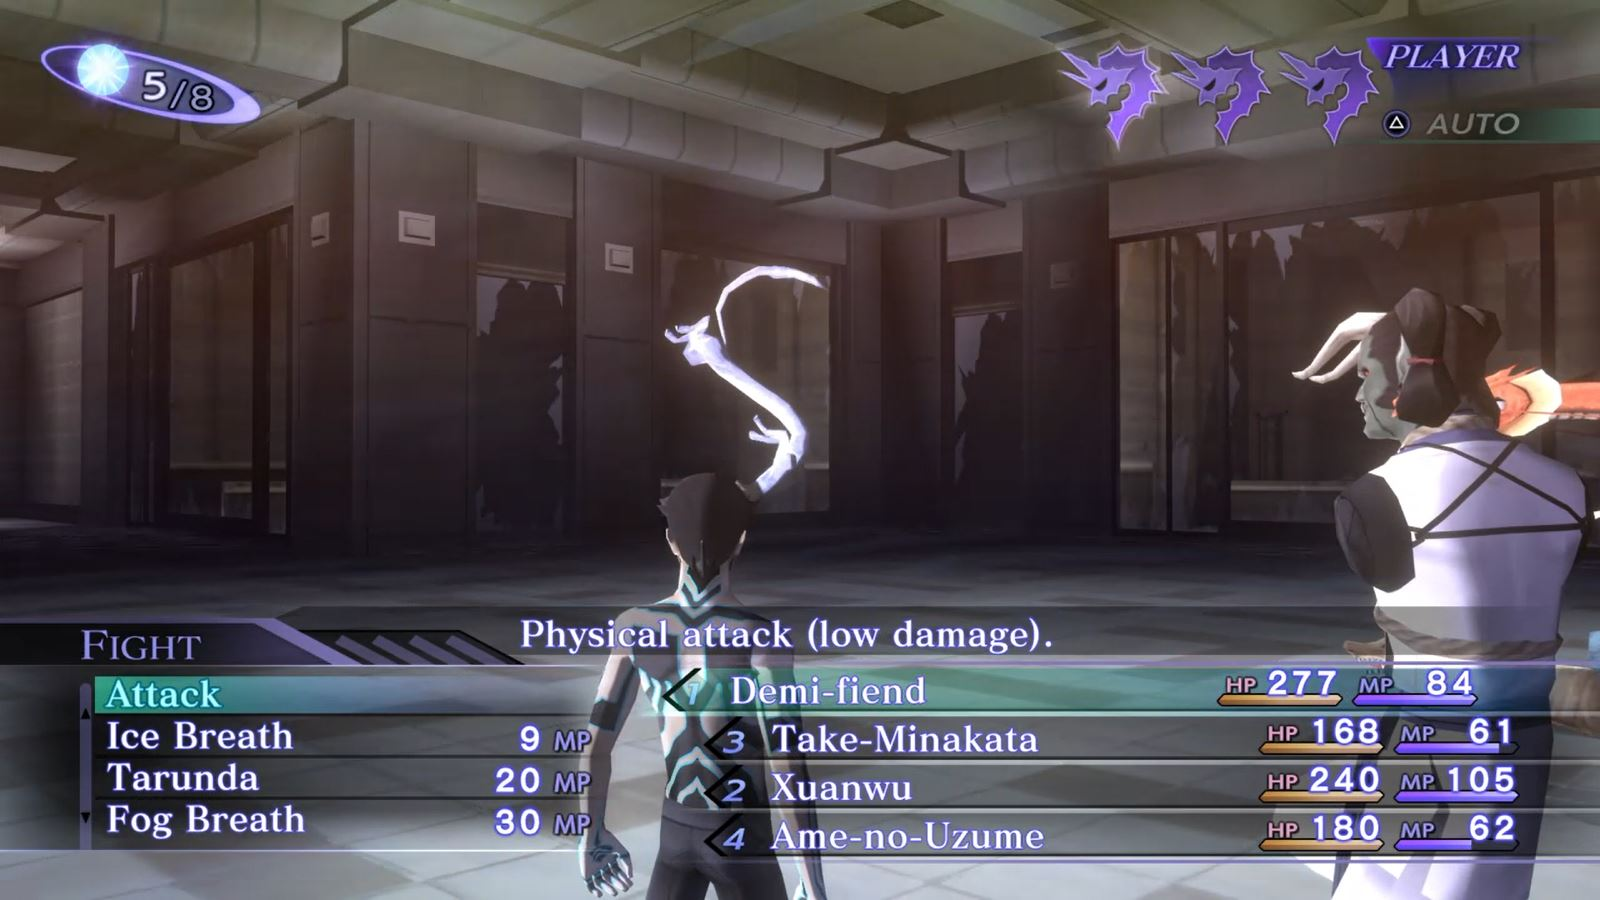
\includegraphics[width=1\textwidth]{smt3_screenshot.jpg}}
  \hfill
  \subfigure[UI sceny walki w projekcie]{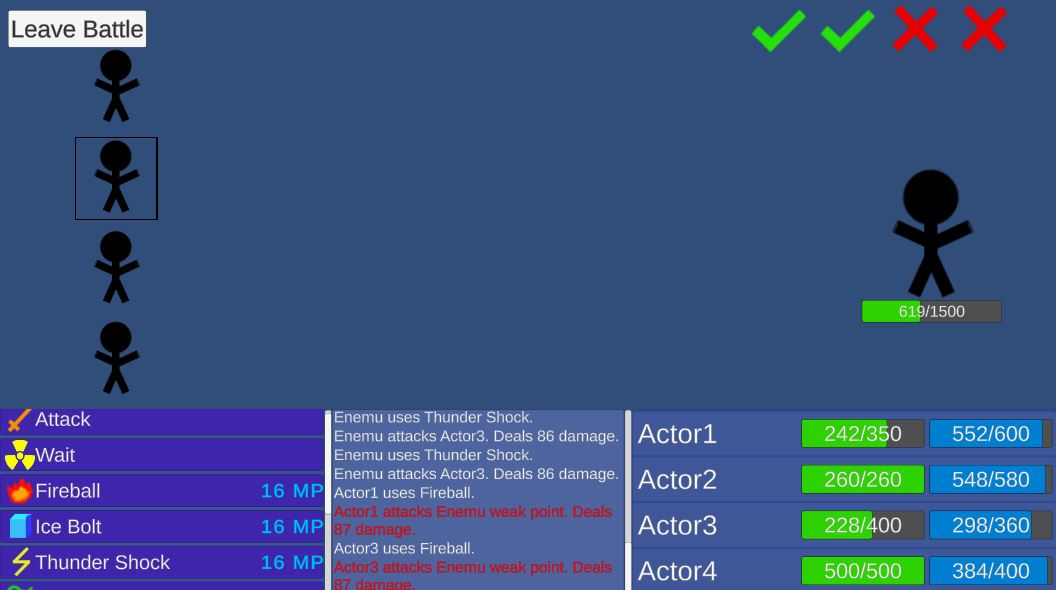
\includegraphics[width=1\textwidth]{battlescreen.JPG}}
  \hfill
  \caption{Zrzuty ekranu porównujące UI stworzone w projekcie do występującego w grze \cite{SMT3}}
\end{figure}
\pagebreak
\subsection{Implementacja systemu Press Turn}
System Press Turn zaimplementowany w projekcie działa na 2 obiektach na scenie BattleScene:
\begin{itemize}
  \item{BattleManager - odpowiada za logikę walki}
  \item{BattleData - przechowuje dane o postaciach, stanach i umiejętnościach}
\end{itemize}
\subsubsection{Zaczytywanie danych oraz startowa konfiguracja obiektów}
Zanim wczyta się scena BattleScene, w kreatorze jest tworzony obiekt BattleData. Przed wypełnieniem go danymi o postaciach posiada listę ze stanami, 
jakich postacie mogą doznać (aktualnie zaimplementowany jest tylko stan Śmierci), oraz listę wszystkich umiejętności. Obiekt jest wypełniany danymi z
kreatora dotyczącymi postaci. Dane te są zapisywane do dwóch list:
\begin{itemize}
  \item{party - przechowująca postaci sterowane przez gracza}
  \item{enemies - przechowująca informacje o postaci przeciwnika}
\end{itemize}
Po wczytaniu się sceny, BattleManager zostaje zainicjowany. Posiada on następujące wartości:
\begin{itemize}
  \item{selectedSkill - przechowuje informacje na temat wybranej przez postać umiejętności}
  \item{isPlayerTurn - wartość prawda/fałsz mówiąca czy rusza się gracz, bazowo ustawiony na prawdę}
  \item{isBusy - wartość prawda/fałsz odpowiadająca za przejście do następnego stadium walki, bazowo ustawiony na prawdę}
  \item{gameState - enumerator mówiący jakie jest stadium walki, może przyjąć jedną z następujących wartości: START\_SIDE, START\_TURN, END\_SIDE, END\_TURN}
  \item{currentCharacter - przechowuje informacje o aktualnie poruszającej się postaci}
  \item{moveQueue - lista z indeksami postaci ułożona w kolejności poruszania się (sortowana po statystyce Agility, od największej wartości do najmniejszej)}
  \item{currentIndex - wartość pomocnicza przechowująca indeks aktualnie poruszającej się postaci}
  \item{turnQueue - lista z wartościami prawda fałsz odpowiadająca ilości tur (zwykłe tury to wartości true, "wciśnięte" tury to wartości false)}
\end{itemize}
\pagebreak
Po wczytaniu wszystkich potrzebnych zasobów, BattleManager ustawia wartości gameState na START\_SIDE oraz isBusy na false.
\subsubsection{Główna pętla systemu walki}
\label{petlagry}
System walki operuje na funkcji Update wykonującej się co klatkę.
\begin{figure}[H]
  \centering
  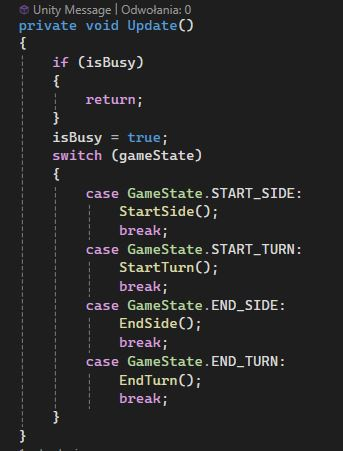
\includegraphics[height=10cm]{updatebattle.JPG}
  \caption{Funkcja Update w obiekcie BattleManager}
  \label{fig:UpdateBattle}
\end{figure}

Funkcja obsługuje tzw. pętle gry czyli algorytm zapętlający rozgrywkę. Pętla gry operuje na wywoływaniu 4 funkcji widocznych na \hyperref[fig:UpdateBattle]{Rysunek 4}. Pętla gry przedstawiona w postaci listy kroków prezentuje się następująco:
\begin{enumerate}
  \item{Wywołuje się StartSide(), które uzupełnia listę tur - turnQueue oraz listę indeksów postaci - moveQueue}
  \item{Następuje aktualizacja currentIndex o pierwszy indeks z moveQueue, przenosząc ten index później na koniec listy moveQueue. Potem zmienia gameState na START\_TURN}
  \item{Wywołuje się StartTurn(), które ustawia wartość currentCharacter na aktualnie poruszającą się postać.}
  \item{Jeśli ruch wykonuje gracz aplikacja pokazuje dostępne umiejętności postaci i czeka na reakcję użytkownika}
  \item{Jeśli ruch wykonuje przeciwnik uruchamiana jest funkcja AIActions() która prosi o podjęcie decyzji wytrenowany model ML-Agents w wyborze celu oraz umiejętności}
  \item{Po wyborze umiejętności i celu wykonuje się funkcja UseSkill() uruchamiająca logikę systemu Press Turn}
  \item{Na koniec gameState jest zmieniany na END\_TURN}
  \item{Wywołuje się EndTurn(), które sprawdza warunki wygranej i przegranej (jeśli któryś z warunków jest prawdziwy, przejdź do 11.)}
  \item{Jeśli turnQueue jest puste, zmień stan na END\_SIDE, w przeciwnym wypadku przejdź do punktu 2.}
  \item{Wywołaj funkcję END\_SIDE, która zmienia wartość isPlayerTurn na przeciwną sobie i zmienia wartość gameState na START\_SIDE. Przejdź do punktu 1.}
  \item{Pokaż ekran końcowy i opuść pętlę gry}
\end{enumerate}

\subsubsection{Działanie funkcji UseSkill() oraz wykorzystanie statystyk postaci}
Wspomniana w pętli gry funkcja UseSkill() pełni kluczową rolę w działaniu systemu walki. Głównym jej zadaniem jest pobranie zasobów (many oraz zdrowia) potrzebnych do użycia wybranej umiejętności, 
aktywacja umiejętności na wybranym celu oraz zmiana tur na podstawie oceny relacji postaci do elementu umiejętności. Gdy dochodzi do aktywacji umiejętności, statystyki postaci atakującej i broniącej są przekazywane do funkcji przeliczającej obrażenia. 
Formuły obrażeń prezentują się nastepująco:
\[PhysicalAttack = 5*\sqrt{\frac{a.Strength}{b.Dexterity}*m}\]\[MagicalAttack = 5*\sqrt{\frac{a.Magic}{b.Dexterity}*m}\]
gdzie,
\begin{itemize}
  \item{a - atakujący}
  \item{b - broniący}
  \item{m - stała moc umiejętności}
\end{itemize}
Jedyna niewykorzystywana nigdzie statystyka to Luck, z uwagi na brak planowanej wcześniej implementacji ciosów krytycznych w systemie walki.
Statystyka Agility jest wykorzystywana do określenia kolejności w kolejce poruszania się postaci.


\section{Część aplikacji automatycznie trenująca model}
Ta część aplikacji służy do trenowania modelu za pomocą pakietu ML-Agents. Składa się z 1 sceny Unity: TrainingScene.

\subsection{Implementacja ML-Agents}
Aby zacząć uczyć model w technice uczenia przez wzmacnianie potrzebne jest środowisko oraz uczący się w nim agent.
\subsubsection{Środowisko}
Środowiskiem jest stworzony wcześniej system Press Turn z którego zostały usunięte niepotrzebne funkcje związane z UI. W rolę gracza wcieli się generator liczb losowych. Będzie on wybierał losową, dostępną umiejętność.
Ilość postaci po stronie gracza jak i statystyki, umiejętności oraz relacje z Elementami będą losowane dla wszystkich postaci. Aby umożliwić powyższe zmieny, dodane zostały następujące elementy do środowiska:
\begin{itemize}
  \label{randomvals}
  \item{turns - ilość minionych tur}
  \item{maxTurns - maksymalna ilość tur po której środowisko powróci do stanu początkowego}
  \item{pointsMin - minimalna wartość wykorzystywana do losowania HP oraz MP postaci. Może przyjąć wartość z zakresu <1,pointsMax)}
  \item{pointsMax - maksymalna wartość wykorzystywana do losowania HP oraz MP postaci. Może przyjąć wartość z zakresu (pointsMin,9999>}
  \item{statMin - minimalna wartość wykorzystywana do losowania statystyk postaci. Może przyjąć wartość z zakresu <1,statMax)}
  \item{statMax - maksymalna wartość wykorzystywana do losowania statystyk postaci. Może przyjąć wartość z zakresu (statMin,99>}
  \item{minActors - minimalna wartość wykorzystywana do losowania ilości postaci po stronie gracza. Może przyjąć wartość z zakresu <1,maxActors)}
  \item{maxActors - maksymalna wartość wykorzystywana do losowania ilości postaci po stronie gracza. Może przyjąć wartość z zakresu (minActors,4>}
\end{itemize}

\subsubsection{Agent}
Implementacja oparta o artykuł~\cite{MLAgentsStartegyGuide}. Aby zaimplementować Agenta za pomocą pakietu ML-Agents należało stworzyć nową klasę dziedziczącą po klasie Agent oraz określić jakie wartości będzie on przewidywał. 
W przypadku tej pracy, Agent będzie przewidywał 2 wartości: 
\begin{itemize}
  \item{Indeks wybranej umiejętności}
  \item{Indeks wybranego aktora}
\end{itemize}
Klasa Agent wymaga do działania nadpisania niektórych swoich metod. Lista przeciążonych metod wraz z opisem nowej funkcjonalności:
\begin{itemize}
  \item{void Heurestic() - z metody została usunięta cała funkcjonalność, przez fakt powodowania niepotrzebnych ostrzeżeń w konsoli Unity. Funkcja pozostaje pusta ze względu na nie używanie jej w projekcie.}
  \item{void CollectObservations() - metoda zajmuje się zebraniem danych ze środowiska oraz wysłanie ich do analizy (spis wszystkich zmiennych branych pod uwagę podczas uczenia został opisany niżej)}
  \item{void OnActionReceived() - metoda odczytuje wybrane przez Agenta wartości i przekazuje je do środowiska}
  \item{void WriteDiscreteMask() - metoda tworzy maskę uniemożliwiającą wybranie przez sztuczną inteligencję umiejętności, do których nie ma dostępu oraz postaci nie żyjących lub nie istniejących}
  \item{void OnEpisodeBegin() - metoda przywraca stan początkowy środowiska w którym się znajduje}
\end{itemize}
\begin{figure}[H]
  \centering
  \subfigure[Funkcja Heurestic() oraz CollectObservations()]{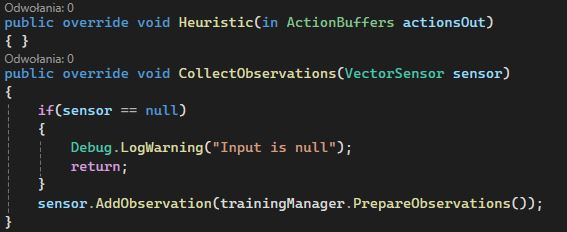
\includegraphics[width=1\linewidth]{Heurestic_Collect.JPG}}
  \hfill
  \subfigure[Funkcja OnActionReceived()]{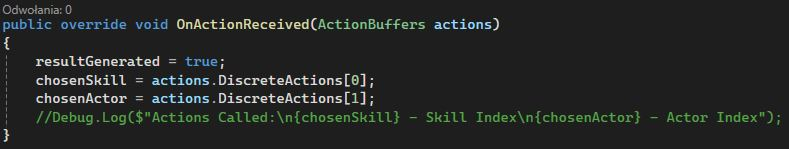
\includegraphics[width=1\linewidth]{OnActionReceived.JPG}}
  \hfill
  \subfigure[Funkcja WriteDiscreteMask()]{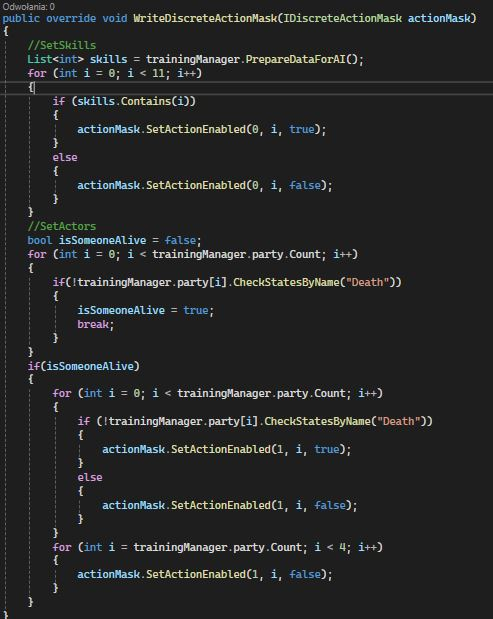
\includegraphics[width=0.70\linewidth]{Mask.JPG}}
  \hfill
\end{figure}
\begin{figure}[H]
  \ContinuedFloat
  \centering
  \subfigure[Funkcja OnEpisodeBegin()]{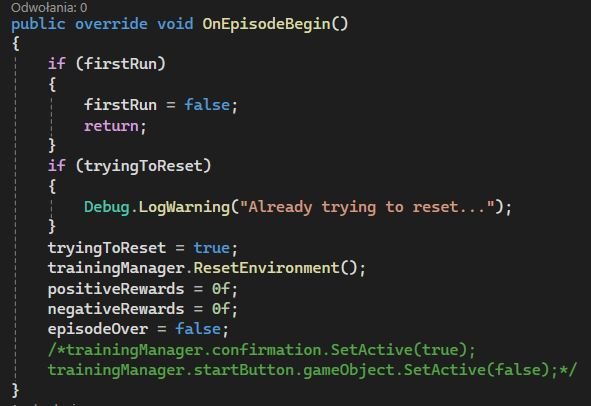
\includegraphics[width=1\linewidth]{Episode.JPG}}
  \hfill
  \addtocounter{figure}{1}
  \caption{Zrzuty ekranu prezentujące ciała nadpisanych funkcji}
\end{figure}
Aby ML-Agents mogło działać poprawnie w systemie turowym, trzeba było dodatkowo wyłączyć Automatyczne Kroki Środowiskowe poprzez funkcję Awake() Agenta. Do ciała funkcji należało wpisać: \verb|Academy.Instance.AutomaticSteppingEnabled = false;|
Powoduje to również konieczność zaimplementowania manualnego wykonywania kroku środowiskowego za pomocą: \verb|Academy.Instance.EnvironmentStep();|
Dodatkowo do klasy zostały zaimplementowane dodatkowe metody oraz właściwości pomocnicze opisane w~\cite{MLAgentsStartegyGuide}. Są to:
\begin{itemize}
  \item{firstRun - wartość prawda/fałsz określająca czy jest to pierwsze wywołanie metody OnEpisodeBegin()}
  \item{tryingToReset - wartość prawda/fałsz informująca, że środowisko jest w trakcie resetu}
  \item{resultGenerated - wartość prawda/fałsz informująca, że model skończył przewidywać wartość i ją zwrócił do środowiska}
  \item{NotifyEndEpisode() - metoda daje nagrodę sztucznej inteligencji za wykonane akcje i kończy epizod}
  \item{GetOutput() - metoda czekająca na to, aż ML-Agents zwróci wynik}
\end{itemize}
\subsubsection{Interakcja środowiska z agentem}
Aby cała struktura uczenia działała, trzeba sprawić aby agent posiadał interakcje ze środowiskiem. W tym celu dostosowano wspomniany w sekcji \nameref{petlagry} algorytm petli gry na potrzeby trenowania modelu.
Nowy algorytm pętli gry wygląda następująco:
\begin{enumerate}
  \item{Wywołuje się funkcja OnEpisodeBegin() i całe środowisko jest na nowo losowane, następnie ustawiana jest wartość gameState na START\_SIDE}
  \item{Wywołuje się StartSide(), które uzupełnia listę tur - turnQueue oraz listę indeksów postaci - moveQueue}
  \item{Następuje aktualizacja currentIndex o pierwszy indeks z moveQueue, przenosząc ten index później na koniec listy moveQueue. Potem zmienia gameState na START\_TURN}
  \item{Wywołuje się StartTurn(), które ustawia wartość currentCharacter na aktualnie poruszającą się postać.}
  \item{Jeśli ruch wykonuje gracz aplikacja losuje umiejętność i cel dla aktualnej postaci}
  \item{Jeśli ruch wykonuje przeciwnik uruchamiana jest funkcja AIActions() która prosi o podjęcie decyzji trenowany model ML-Agents w wyborze celu oraz umiejętności. Po otrzymaniu wyniku wykonuje się funkcja EnvironmentStep()}
  \item{Po wyborze umiejętności i celu wykonuje się funkcja UseSkill() uruchamiająca logikę systemu Press Turn}
  \item{Na koniec gameState jest zmieniany na END\_TURN}
  \item{Wywołuje się EndTurn(), które sprawdza warunki wygranej, przegranej oraz limitu tur (jeśli któryś z warunków jest prawdziwy, przejdź do 12.)}
  \item{Jeśli turnQueue jest puste, zmień stan na END\_SIDE, w przeciwnym wypadku przejdź do punktu 3.}
  \item{Wywołaj funkcję END\_SIDE, która zmienia wartość isPlayerTurn na przeciwną sobie i zmienia wartość gameState na START\_SIDE. Przejdź do punktu 2.}
  \item{Wywołaj funkcje NotifyEndEpisode(), która daje nagrodę dla modelu i powoduje przejście do punktu 1.}
\end{enumerate}
\pagebreak
\subsubsection{Zmienne wybrane do uczenia}
\label{zmienne}
Zmiennych uczących jest łączne 87. W ich skład wchodzą:
\begin{enumerate}
  \item{Ilość zwykłych tur}
  \item{Ilość "wciśniętych" tur}
  \item{Statystyki Aktora 1 - 17 zmiennych}
  \item{Statystyki Aktora 2 - 17 zmiennych}
  \item{Statystyki Aktora 3 - 17 zmiennych}
  \item{Statystyki Aktora 4 - 17 zmiennych}
  \item{Statystyki Przeciwnika - 17 zmiennych}
\end{enumerate}
Wszystkie zmienne są poddane normalizacji według wzoru:
\[normValue = \frac{value-minValue}{maxValue-minValue}\]
W przypadku gdy aktor nie został stworzony w danym epizodzie, wszystkie 17 przypisanych do niego zmiennych przyjmuje wartość 0.
\subsection{UI}
\begin{figure}[H]
  \centering
  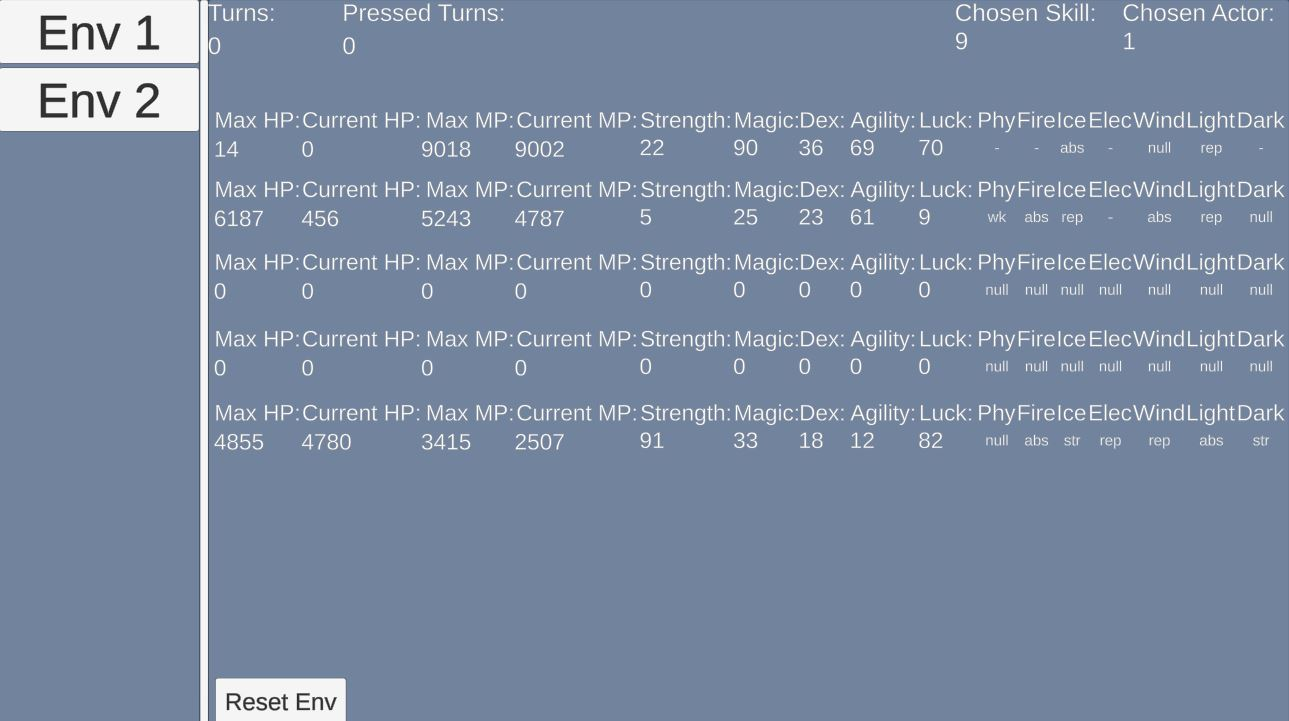
\includegraphics[height=8cm]{trainingui.JPG}
  \caption{Widok UI do nadzoru trenowania modelu}
\end{figure}
\pagebreak
Widok składa się z 2 elementów:
\begin{enumerate}
  \item{Listy środowisk}
  \item{Panelu szczgółowego}
\end{enumerate}
Elementy te są ze sobą głęboko powiązane. Po naciśnięciu przycisku w liście środowisk, panel szczegółowy zmienia pokazywane dane na te z wybranego środowiska.
Panel szczegółowy pokazuje wszystkie zmienne w nieznormalizowanej postaci. Są one ustawione w taki sam sposób jak to opisuje lista w sekcji \nameref{zmienne}.
Ponadto wyświetlane są ostatnio wybrane wartości przez sztuczną inteligencję w postaci indeksów poszczególnych danych. Dostępny jest również przycisk restartu
środowiska Reset Env, przywracający je do stanu początkowego.

\chapter{Instrukcja instalacji i korzystania}
\section{Instalacja}
\subsection{Wymagane programy}
Aby aplikacja była poprawnie uruchamiana potrzebne są określone komponenty. W przypadku wersji nowszych/starszych od podanych nie ma gwarancji prawidłowego działania aplikacji.
Lista potrzebnych komponentów:
\begin{itemize}
  \item{Unity Hub - używany do instalacji silnika Unity}
  \item{Unity wersja 2022.2.11f1 - program Unity Hub sam zapyta o zainstalowanie tej wersji silnika podczas pierwszej próby uruchomienia projektu}
  \item{Python v3.9.13}
  \item{(opcjonalnie) Visual Studio 2022 lub Visual Studio Code - do edycji kodu źródłowego aplikacji}
\end{itemize}

\subsection{Konfiguracja wirtualnego środowiska Pythona}
Wirtualne środowisko umożliwia instalacje pakietów bezpośrednio w folderze z projektem, dzięki czemu może on zostać zabrany na przenośny dysk i uruchomiony na każdym komputerze posiadającym wymienione wczesniej komponenty.
Poniższa instrukcja jest napisana z myślą o systemie operacyjnym Windows, gdyż na tym systemie aplikacja była tworzona i testowana.
Aby skonfigurować wirtualne środowisko, należy:
\begin{enumerate}
  \item{Uruchomić Wiersz Poleceń (cmd) w folderze bazowym projektu}
  \item{Sprawdzić za pomocą wiersza poleceń swoją wersję Pythona za pomocą polecenia:
  \begin{lstlisting}
  python
  \end{lstlisting}
  jeśli jest poprawnie zainstalowany, zostanie otworzony program Python CLI pokazujący zainstalowaną wersję Pythona. Aby z niego wyjść należy użyć komendy:
  \begin{lstlisting}[language=Python]
  exit()
  \end{lstlisting}
  }
  \item{Utworzyć wirtualne środowisko za pomocą komendy:
  \begin{lstlisting}
  python -m venv venv
  \end{lstlisting}
  }
  \item{Aktywować wirtualne środowisko w wierszu poleceń za pomocą polecenia:
  \begin{lstlisting}
  venv\Scripts\activate
  \end{lstlisting}
  }
  \item{Zainstalować narzędzie pip do wirtualnego środowiska odpowiadające za pobieranie pakietów Pythona wpisując:
  \begin{lstlisting}
  python -m pip install --upgrade pip
  \end{lstlisting}
  }
  \item{Za pomocą narzędzia pip pobrać pakiet ML-Agents wpisując:
  \begin{lstlisting}
  pip install mlagents
  \end{lstlisting}
  }
  \item{Zainstalować pakiety wchodzące w skład biblioteki PyTorch wpisując:
  \begin{lstlisting}
  pip install torch torchvision torchaudio
  \end{lstlisting}
  }
  \item{Zmienić wersję pakietu protobuf, gdyż ta instalowana razem z ML-Agents nie działa poprawnie, za pomocą komendy:
  \begin{lstlisting}
  pip install protobuf==3.20.3
  \end{lstlisting}
  }
  \item{Pobrać pakiet ONNX odpowiadający za tworzenie plików przechowywujących modele wpisująć polecenie:
  \begin{lstlisting}
  pip install onnx
  \end{lstlisting}
  }
  \item{Sprawdzić, czy ML-Agents zostało poprawnie zainstalowane za pomocą komendy:
  \begin{lstlisting}
  mlagents-learn -h
  \end{lstlisting}
  }
\end{enumerate}

\section{Korzystanie z aplikacji}
\subsection{Uruchomienie trenowania modelu}
Pierwszym etapem jaki trzeba wykonać jest wytrenowanie modelu. Aby to zrobić trzeba wykonać nastepujące kroki:
\begin{enumerate}
  \item{Uruchomić projekt poprzez Unity Hub}
  \item{Otworzyć scenę TrainingScene znajdującą się w folderze Assets/Scenes}
  \item{Na panelu Hierarchy należy wyszukać obiekt Environments. Służy on do przechowywania Środowisk uczących model}
  \item{Zklonować obiekt Environment będący dzieckiem obiektu Environments tyle razy, ile ma być środowisk uczących}
  \item{Skonfigurować Środowiska. Obiekt TrainingManager służy do konfiguracji losowych statystyk postaci w środowisku, a MLAgentsTrainer ustawia wartości nagród za akcje}
  \item{Uruchomić wiersz poleceń w folderze z projektem następnie aktywując wirtualne środowisko}
  \item{Uruchomić ML-Agents za pomocą komendy:
  \begin{lstlisting}
  mlagents-learn
  \end{lstlisting}
  Natomiast, jeśli już wcześniej model był uczony możemy zmusić ML-Agents do ponownego uczenia wpisując:
  \begin{lstlisting}
  mlagents-learn --force
  \end{lstlisting}}
  \item{Gdy ML-Agents wyświetli komunikat w którym czeka na Unity, należy uruchomić scenę TrainingScene w Unity za pomocą funkcji playtest}
  \item{Gdy będziemy uważać, że model jest dostatecznie wytrenowany, należy wpierw opuścić playtest, a następnie w zatrzymać uczenie w wierszu poleceń za pomocą skrótu CTRL+C.
  Po zatrzymaniu, ml-agents wyświetli nazwę oraz ścieżkę do pliku z rozszerzeniem .onnx w której model został zapisany}
\end{enumerate}
Wszystkie pliki wynikowe ML-Agents znajdują się w folderze results/ppo/. Jest możliwość uruchomienia aplikacji Tensorboard, aby obserwować przebieg uczenia, lecz z uwagi na to, 
że pakiety wykorzystywane przez ML-Agents są przestarzałe, nie są kompatybilne z pakietami wymaganymi przez pakiet Tensorflow (potrzebny do działania aplikacji Tensorboard) wykorzystujący te same pakiety, ale w nowszej wersji.
Po próbach instalacji starszych wersji pakietów, nie udało się uzyskać działającej aplikacji Tensorboard, przez co finalnie nie jest dostępna w implementacji.
\pagebreak
\subsection{Uruchomienie symulacji}
Po wytrenowaniu modelu, trzeba go przypisać do sztucznej inteligencji na scenie z symulacją. Aby to zrobić należy wykonać następujące kroki:
\begin{enumerate}
  \item{Skopiować plik z modelem o ścieżce podanej po zakończeniu uczenia do folderu Brains znajdującego się w katalogu [Ścieżka Projektu]/Assets/Data/}
  \item{Otworzyć scenę BattleScene znajdującą się w folderze Scenes}
  \item{Do obiektu MlAgentsAI należy przypisać wytrenowany model. Robi się to przeciągając z widoku folderów projektu plik o rozszerzeniu .onnx do właściwości Model obiektu MlAgentsAI}
  \item{Otworzyć scenę MainMenu i uruchomić symulację}
\end{enumerate}
Po tych krokach można dostosować statystyki postaci gracza oraz przeciwnika i zasymulować walkę na danym modelu.

\subsection{Sposób oceny modelu}
Z uwagi na wcześniej wspomniany brak możliwości implementacji aplikacji Tensorboard, nie da się dokładnie sprawdzić jakości modelu. Można jednak sprawdzić czy model dokonuje poprawnych decyzji podczas różnych prób symulacji.
W moim przypadku oceniałem czy model po zobaczeniu słabości na jakiś konkretny żywioł np. Ogień, posiadając też inne dostępne umiejętności będzie bardziej skłonny do atakowania tym typem obrażeń. 

\chapter{Wnioski}
W mojej ocenie, oparcie sztucznej inteligencji w grach na przetrenowanych modelach jest w obecnych czasach możliwe. Problemem jest dodatkowe dotrenowanie lub całkowite trenowanie od podstaw modelu podczas trwania gry.
ML-Agents wymaga uruchomionego środowiska Unity, które jest edytorem gry, aby móc trenować model co wyklucza taką możliwość. Jednak technologie uczenia maszynowego rozwijają się bardzo prężnie i jak jeszcze w roku 2020 technologie
uczenia maszynowego były domeną naukową, bardzo mało znaną poza tym kręgiem, to aktualnie są bardzo ważną i dynamicznie rozwijaną dziedziną. Może to spowodować na tyle duży rozwój tej technologii, że uczenie sztucznej inteligencji
podczas gry będzie możliwe.


\begin{thebibliography}{9}
  \bibitem{MachineLearningTypes}
  Shagan Sah,
  \textit{Machine Learning: A Review of Learning Types},
  (2020 r.)

  \bibitem{ReinforcementLearning}
  Vincent François-Lavet, Peter Henderson, Riashat Islam, Marc G. Bellemare, Joelle Pineau,
  \textit{An Introduction to Deep Reinforcement Learning},
  (2018 r.)

  \bibitem{MLAgentsDocs}
  \textit{Unity ML-Agents Toolkit Documentation} 
  \url{https://unity-technologies.github.io/ml-agents/ML-Agents-Toolkit-Documentation/}
  (dostęp 06.01.2024r)

  \bibitem{UnityDocs}
  \textit{Unity Documentation}
  \url{https://docs.unity.com}
  (dostęp 06.01.2024r)

  \bibitem{GodotDocs}
  \textit{Godot Documentation}
  \url{https://docs.godotengine.org/en/stable}
  (dostęp 06.01.2024r)

  \bibitem{GodotRLAgentsArticle}
  Edward Beeching, Jilles Debangoye, Olivier Simonin, Christian Wolf,
  \textit{Godot Reinforcement Learning Agents},
  (2021 r.)

  \bibitem{GodotRLAgentsDocs}
  \textit{Godot RL Agent Repository}
  \url{https://github.com/edbeeching/godot_rl_agents}
  (dostęp 06.01.2024r)

  \bibitem{UnrealDocs}
  \textit{Unreal Engine Documentation}
  \url{https://docs.unrealengine.com}
  (dostęp 06.01.2024r)
  
  \bibitem{PPOArticle}
  John Schulman, Filip Wolski, Prafulla Dhariwal, Alec Radford, Oleg Klimov, 
  \textit{Proximal Policy Optimization Algorithms},
  (2017 r.)

  \bibitem{SACArticle}
  Tuomas Haarnoja, Aurick Zhou, Pieter Abbeel, Sergey Levine, 
  \textit{Soft Actor-Critic: Off-Policy Maximum Entropy Deep Reinforcement Learning with a Stochastic Actor},
  (2018 r.)

  \bibitem{RLLearningInTBRPG}
  SangGyu Nam, Kokolo Ikeda,
  \textit{Generation of Diverse Stages in Turn-Based RolePlaying Game using Reinforcement Learning}
  (2019 r.)

  \bibitem{PlayerPreferencesInRPGs}
  Ville Mäkelä, Albrecht Schmidt,
  \textit{I Don’t Care as Long as It’s Good: Player Preferences for
  Real-Time and Turn-Based Combat Systems in Computer RPGs}
  (2020 r.)

  \bibitem{SMT3}
  Atlus,
  \textit{Shin Megami Tensei III},
  (2003 r.)

  \bibitem{MLAgentsStartegyGuide}
  Andrew Zuo,
  \textit{Guide On Using Unity ML Agents For A Turn Based Strategy Game},
  (2021 r.),
  \url{https://andrewzuo.com/guide-on-using-unity-ml-agents-for-a-turn-based-strategy-game-9e52e6945a31} 
  (dostęp 06.01.2024r)
\end{thebibliography}

\beforelastpage

\end{document}